\chapter{Urban Land and Land Rent} \label{chapter-space}

\epigraph{Overall, several decades after its creation, the standard urban model seems to still capture surprisingly well the inner structure of many cities across the world, both in developed and in developing countries.}{Liotta et al. 
 \cite{liottaTestingMonocentricStandard2022}}

%MAKE ALONSO A CHARACTER, AND INTRODUCE HIS PROBLEMS
% A large part of the surplus appears as locational rents, so we then go to developing the spatial and urban model in which rent operates.  
% URBAN MODELS ARE ROOTED IN CLASSICAL NOTIONS OF RENT, FOLLOW A SIMILAR LOGIC TO RICARDOS EARLY AGRICULTURAL MODEL.
% WHAT ARE THEY MODELLING
% WHAT QUESTIONS WERE THEY DEVELOPED TO EXPLORE/ANSWER
% WHAT IS THE CONTEXT/PERIOD/SOCIETAL CONDITIONS THAT PROVIDED THE CONTEXT FOR THESE TO EMERGE IN? 
% DOES WEALTH/RENT/PRODUCTION FIT INTO THE MODEL? WHAT IS INCLUDED BEFORE WHAT IS NOT INCLUDED
% SOMETHING LIKE RENT OR RELATED TO RENT SEEMS TO BE PART OF THEM... DID THIS COME FROM RENT? OR TO ANSWER SIMILAR QUESTIONS? OR DOES IT COME FROM A DIFFERENT DIRECTION BUT MODEL SIMILAR? 
% WERE THEY ANSWERING THE SAME QUESTIONS
% WHAT WERE THE QUESTIONS ABOUT CITIES AND SPACE THEY WERE TRYING TO ANSWER? 
% WHAT SPECIFIC SPATIAL.URBAN FEATURES WERE IN THE MODELS

% The s tudy of space is huge, and seeping into those few fields it hasn't infiltrated. 

% Urban modelling, done by planers geographers and econoists. It tends to focus on transportation, the study of space. The fiedl is space. locations of people, housing forms, the demographic and form of the field

% urban modelling is a sub discpline. There ar programs of urban economic it's a subfield of regional science/regional economics.

% Modeling location, spatial value, locations represents a sub-feids in regional science and a sub-field in economics. A model which brings the two closer together is the Alonso model. It's dominant feature.

% DON'T EXPLAIN WHAT AN URBAN MODEL IS AT ALL. WHAT IS THE CONTEXT, WHAT QUESTIONS ARE THEY TRYING TO ANSWER. 
% SOUNDS LIKE THEY ARE TRYING TO DO THE SAME THINGS AS ECONOMISTS DO WITHOUT THE SAME TOOLS. 
% THEY DON'T HAVE THE SAME PROBLEMS.


The early 1960s were a watershed in urban economics. Land rent theory returned to economics and \gls{regional science} in the form of a new model of urban structure  that linked the urban wage premium to urban land rents through transportation costs. The model rapidly became the workhorse for theorists and empirical researchers. It helped explain land prices, the built form of the city, and where people live relative to where they work, using a logic analogous to Ricardo's theory of rent, as it appeared in the story of the carter carrying farm products to market in Section~\ref{section-rent-carter}), applying it to a city where workers commute to jobs. % (TRIED EXPLAINING A FEW OF THE THINGS IT GAVE INSIGHT TO  MAKE THIS MORE CONCRETE, BUT IT MIGHT BE BETTER TO MENTION SOMETHING ELSE?)


The goal of this chapter is to describe informally the now classic and dominant spatial urban model that that emerged at that time. It serves in our analysis as the link between rent theory and financialization. % we will use. 
We will review the theory and development of the core urban model and discuss how it uses urban land rent to explain urban size and structure. % to our analysis. These models 

THIS IS AMAZING!! 
MAYBE NOTE THAT IT DIDN'T BRING FORWARD DISTRIBUTIONAL ASPECTS HERE?
I THINK IT WOULD HELP TO SAY WHAT REGIONAL SCIENCE IS/HOW IT IS DIFFERENT FROM URBAN ECONOMICS.

What we refer to the basic model is often called the Alonso model, although it  was developed by several scholars working in parallel in parallel in roughly the same period. William Alonso published \textit{Location and Land Use} in 1964  \cite{alonsoLocationLandUse1964} based on his 1960 PhD thesis \cite{alonsoModelUrbanLand1960},  
giving him a slender priority in the literature. 
Richard Muth's \cite{muthSpatialStructureHousing1961}, and \cite{muthRationalExpectationsTheory1961} were written roughly simultaneously with and independently of Alonso's thesis, and culminated in Muth's classic book, Cities and Housing  \cite{muthCitiesHousingSpatial1969}.\footnote{See ``William Alonso, Richard Muth, Resources for  the Future, and the founding of urban economics''\cite{mcdonaldWilliamAlonsoRichard2007} for a more detailed discussion of the development of the model.}  % ***E ADD % This workoverlps with Alonso in these ways. Differed in these ways \dots USE THIS TO FLESH OUT MORE OF THWAT HIS MODEL?WORK ISDOING AND HOW
% We will refer to the core urban model developed by 
 The model was developed further by Muth \cite{muthCitiesHousingSpatial1969} and Mills \cite{millsAggregativeModelResource1967}, and later formalised by Wheaton \cite{wheatonComparativeStaticAnalysis1974}.\footnote{it is also called the Alonso model, the Alonso-Muth model, the Alonso-Muth-Mills model, the circular city model, and the monocentric city model.} %(***E ADD \dots % He was concerned with \dots His model did \dots INTRODUCE THE WORK ITSELF) 
\footnote{It is worth noting that Lowdon Wingo also had what appears to be a working paper, \textit{Transportation and Urban Land} \cite{wingoTransportationUrbanLand1961}, for the organization Resources for the Future  in preparation for publication that presented a core idea and  significantly influenced Muth \cite{mcdonaldWilliamAlonsoRichard2007}.} Mills' \textit{Urban Economics} \cite{millsUrbanEconomics1972}. followed soon after. 

The model is built around an extremely simple trick for calculating what people will bid or pay to live at a particular location relative called the \gls{bid-rent curve}. Starting with the fact that a worker is more productive in the city, the worker should receive a wage premium, $\omega$ for working in the city. That premium has to cover the cost of commuting to work, so there is  a part of the  wage premium left as a benefit for the urban worker. 

But notice this additional point: if workers are renting their homes, landlords can charge a premium for being closer to the center of the city where transportation costs are lower.  Landlords can capture a share of urban productivity. How much can they charge? How much will a worker bid for a rental? The maximum charge is the part of the wage premium left after transportation costs are paid. If landlords are at all greedy, that is also the minimum they will charge. 

We can write a very simple formula for the maximum  bid: 
\begin{equation}  
\mathcal{R}= \omega - dc \label{eqn-bid-rent}\end{equation}
where $d$ is the distance from work and $c$ is the transportation costs.\footnote{ if the wage is paid monthly then $c$ has to be the monthly transportation cost.} Equation~\ref{eqn-bid-rent} describes a downward-sloping line (a curve) that is known as the bid-rent curve.


The seeds of the \gls{bid-rent curve} that is  at the heart of the model were presented as early as 1885  by German engineer-economist Wilhelm Launhardt \cite{blaugEconomicTheoryRetrospect1985, launhardtMathematischeBegruendungVolkswirthschaftslehre1885}. The  \gls{bid-rent function} was first applied explicitly to the equilibrium of land use patterns in agricultural production by August Losch \cite{loschEconomicsLocation1954} in Germany and later by Edgar S. Dunn \cite{dunnEquilibriumLandUsePatterns1954} in America. It was not until the 1960s that it was discovered that it could be applied  to the urban setting by Alonso and others. It was then very quickly recognized as a fraternal twin of August von Th\"unern's 1826 agricultural planning model \cite{vonthunenIsolirteStaatBeziehung1826}. With the work of Alonso and his contemporaries, the concept of land rent had moved  from  agricultural economics to the centre of the modern urban economy.  


% https://press.uchicago.edu/ucp/books/book/distributed/C/bo23348570.html Macy Conference
% https://archives.library.illinois.edu/thought-collective/cybernetics-thought-collective/
% Norbert Wiener published Cybernetics in 1948
% Margaret Mead and Gregory Bateson


% "The Macy Conferences on cybernetics brought together a diverse host of scholars, including Margaret Mead and Gregory Bateson (anthropology), Warren S. McCulloch (neurophysiology), Heinz von Foerster (physics and electrical engineering), Norbert Wiener (mathematics), W. Ross Ashby (psychiatry), John von Neumann (computer science), Claude Shannon (mathematics and electrical engineering), G. Evelyn Hutchinson (ecology), and Arturo Rosenblueth (physiology). While these scholars met together at the conferences on a few rare occasions, they used a variety of other means to create and foment a community—a Denkkollektiv, or a scientific “thought collective”—around cybernetics. As defined by scientist Ludwik Fleck in his influential publication Genesis and Development of a Scientific Fact, a thought collective is a “community of persons mutually exchanging ideas or maintaining intellectual interaction” (Fleck, 1979), and the cybernetics thought collective subsisted during the three decades that followed the Macy Conferences.

Rent emerges from the %essential 
scarcity of space, and models exploit relationship between rent and location  described in  Equation~\ref{eqn-bid-rent} to explore the spatial structure of the city. 
 Bruckner \cite{bruecknerStructureUrbanEquilibria1987} describes the resulting model as ``a simple yet powerful model of urban spatial structure that successfully explains the principal regularities observed in the urban landscape,'' and goes on to say ``the good predictive performance of the model suggests that its simplifications are artfully chosen, capturing the essential features of real-world cities.'' It remains the central model in modern urban economics.

The models don't however bring forward the distributional and class features derived by the classical economists. They don't examine distribution or how the distribution of rents might affect the productivity of the city, which means they throw no light on the effects of financialization of the property market on distribution or on urban productivity. 
In this thesis we  explore who gets the urban land rents and how that is changed by the financialization of urban housing.

% Standard urban models are based on spatial rents, and follow directly from the theory of rent developed in Ricardo.
% As discussed in the previous chapters, 
% Modern urban models apply classical rent theory to understanding the structure of the city. %are essentially an application of classical rent theory. 


% HENRY GEORGE applied to cities, urban models formalized the concept.
% Although the model is easily generalized, we restrict our presentation to the highly stylized core version to establish how land rents are generated in the urban system and how they are related to neoclassical growth theory. 


% \section{From Ricardo's rent to Alonso's urban model}

% The Alonso model extends the approach developed in Ricardo approach to rent to the urban system, and is % Alonso's spatial model is 
% rooted in the classical notion of rent. 



\section{From Ricardo's rent to Alonso's urban model}
The Alonso model extends the approach developed in Ricardo approach to rent to the urban system, and is rooted in the classical notion of rent. Alonso, however, re-presents Ricardo's conception of rent mathematically for a different social system and production technology. Ricardo had described a model with a central market for an agricultural product like potatoes, producing potatoes took land and transporting potatoes to market was costly. Because there is one market price for potatoes, land with low transportation costs near the central market earns a rent. More distant land has lower value. In Alonso's model there is central market and a single price for labour, producing labour takes land, and transporting labour to the market is costly. 





Figure~\ref{fig-alonso-simple} illustrates the simplest case. we are looking at a thin slice of the city from the centre to its edge at $d^*$. The vertical dimension is dollars of rent or trasportation cost.  Notice that they sum to $\omega$. 

We assume in theis simple model that the city sits on a uniform plane and has a population of identical workers with identical housing needs, and identical transportation costs who all work at the city centre and receive the same wage. We also assume, as is common for simple versions of the model, that the labour market and production sector at the centre take no space. 

As above, transportation to and from the center costs ${c}$ times the distance $d$ from the center.\footnote{Fuel, capital, and time costs are  all included in the transportation costs, ${c}$. } The diagonal line is the bid-rent curve. The figure shows  bid-rent declining with distance from the centre and transportation cost rising. Property values at any point are a multiple of the rent at that point. 

At $d^*$ transportation costs completely absorb the wage premium. There is no surplus that the landlord can extract.\footnote{In many discussions of the model it is assumed that beyond $d^*$ the best use of the land is for agriculture since it cannot earn a rent premium. }

% %%%%%%%%%%%% PARTITIONING THE LABOUR SHARE
\begin{figure}[!ht]
    \begin{center}
    
% Simple Alonzo model
%%%%%%%%%%%%%%%%%%%%%%%% PARTITIONING THE LABOUR SHARE
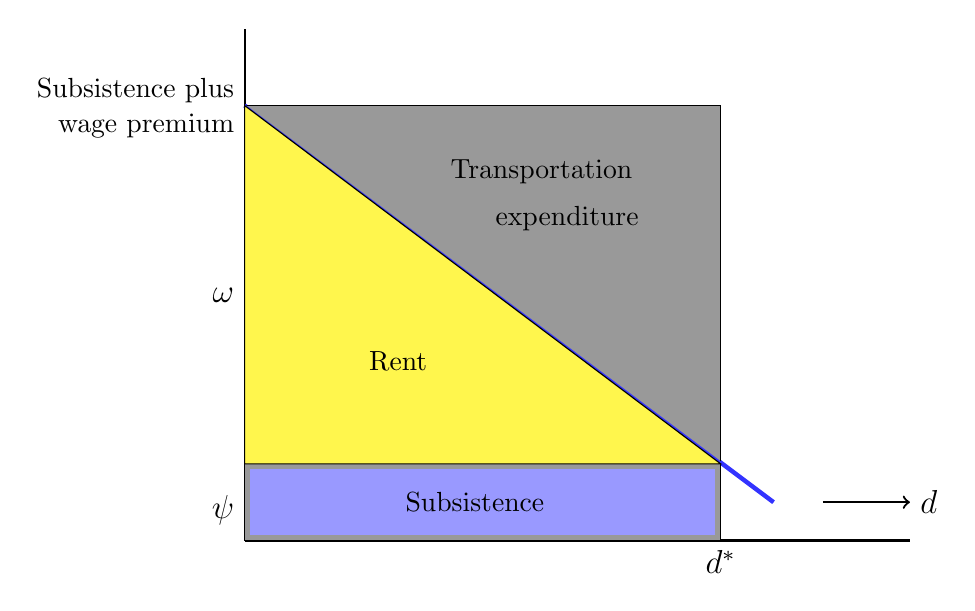
\begin{tikzpicture}[scale=.65]
\def\bndmax{5}        %https://tex.stackexchange.com/questions/68462/filling-a-complex-region-with-tikz
\def\bndmin{0.2}
\def \n {8.5}  % height of y axis
\def \d {13}  % length  of x axis
\def \t {.75}  %  cost of transportation per unit x
\def \th {1}   %
\def \w {7}    %  wage premium
\def \om{1.5}%  omega =rural wage Zero for urban population
\def \azero{2}
\def \aprime {-.0}	
\tikzset{func/.style={thick,color=blue!80}}	

% FIRST FIGURE just axes PARTITIONING THE LABOUR SHARE
\draw [thick] (0,-\om) --(\d,-\om);  			% Zero for rural population
\draw [thick] (0,-\om) --(0,\n); %node[above]{\Huge $w$};	% Y axis
%\node at (0,\n+0.5){\large $Rent$};

% \draw [thick] (0,0)node[left=.5]{Subsistence}--(\d,0);
%\node at(-2,1) {$\omega$};
\node[left=.25] at (0,3.3){\large $\omega$};
\node[left=.25] at (0,-0.9){\large $\psi$};
%\node[left=.25] at (0,3){$w+\omega$};
\node[left=.25] at (0,\w+.3){Subsistence plus};
\node[left=.25] at (0,\w-.4){wage premium};	

%\foreach \xi in {0,..., \n} \draw (\xi,0)--(\xi,-.1)node[below=1]{\small$\xi$};
%\foreach \yi in {1,...,\n} \draw (0,\yi)--(-.1,\yi)node[left]{$\yi$};
%\foreach \i in {1,4,9,16} {
%\node at (7,-\om/2){people scattered uniformly across the land  };

%SECOND FIGURE WITH AGGLOMERATION WAGE
%   \pause %  add urban production and net wage PARTITIONING THE LABOUR SHARE
%\draw[fill=white, white] (0.1,-0.1) rectangle (14,-\om+.1);
%\draw [fill=green!80] (-.25, 0) rectangle(.25, \w);
\node[right] at  (.25, \w/2){Added Productivity};
% \node[right, text width = 3cm] at  (10,9){Where does the increase in productivity come from?};
\draw [ thick, ->](11.3,-\om/2)--(13, -\om/2)node [right] {\large $d$};

%  THIRD FIGURE  add wage profile PARTITIONING THE LABOUR SHARE
% \pause
%\node[right, white, fill=white,  text width = 3cm] at  (10,9){Where does the increase in productivity come from?};
\draw[func, domain=0:\w/\t+1,ultra thick] plot [samples=200] (\x,{\w-\t*\x}); %Net wageprofile  for 
%\node[right, white, fill=white] at  (.25, \w/2){Added Productivity};
%\node[right, fill=white, text width =3.5cm ] at  (1, \w/2){Declining wage  net \\of transportation\\ costs $T(d)$ };

%   FOURTH FIGURE     commuters PARTITIONING THE LABOUR SHARE
%\pause
%\draw[fill=blue!40] (0.1,-0.1) rectangle (9.2,-\om+.1);
%\node at (4.5,-\om/2){commuters};

%   FOURTH FIGURE    wage bill
%\pause %add total new value
% \draw[fill=green!40] (0,-\om) rectangle(9.30,\w);% new product
% \node at (4.5,\w/2){\Large urban wage bill};

%%   FIFTH FIGURE   distribution
%\pause
%\node at (9,\n){\Large Partitioning the Labour Share};

\draw[fill=black!40] (0,-\om) rectangle (9.30,\w);% new product repeat
\draw[func, domain=0:\w/\t+1] plot [samples=200] (\x,{\w-\t*\x}); %rent profile
\fill[blue!40] (0.1,-0.1) rectangle (9.2,-\om+.1);
\node at (4.5,-\om/2){Subsistence};
\draw[fill=yellow!70,] (0.,0.) -- (0,7)--(9.30,0.)--cycle;% Rent \w-.2
\node at (3.,2){Rent}; 		%Rent 
\node at (5.8,5.7){Transportation};
\node at (6.3,4.8){expenditure};
\node at (9.3,-1.5)[below]{ \large $d^*$};
% \node at (4.8,\w)[above]{\huge $d^*$};
 \end{tikzpicture}
 

    \caption[The allocation of worker income by distance from the centre of the city.]{The allocation of worker income by distance from the centre of the city, where $\psi$ represents the \gls{subsistence wage}, which is the same as the rural income, and $\omega$ represents the \gls{urban wage premium}, which is paid out of the increased urban productivity resulting from agglomeration.}
    \label{fig-alonso-simple}
    \end{center}
\end{figure}

 The figure describes a locational equilibrium among mobile households. Since individuals would simply move to any location that offered a higher utility, in an equilibrium all the otherwise identical workers must receive the same utility. This has to be the case even though those farther from the center must pay more for transportation to and from home. The variable that  adjusts to maintain equal utility with rising transportation spending is the cost of housing. This conception of a \gls{locational equilibrium} is the heart of the model and all its extensions.\footnote{For economists it is also described as a Nash equilibrium.}

In Figure~\ref{fig-alonso-simple}, the height of yellow triangle  represents the wage premium $\omega$ for urban labour and the amount land rent earned at the centre % of the city.  at the centre, 
where transportation costs are zero. The entire yellow triangle is aggregate land rent generated by the city along a section from the centre to the edge. The model says nothing about who gets the rent in the urban economy. For classical economists it was obvious that the agricultural rents went to the class of land-owners, as discussed in Chapter~\ref{chapter-rent}. For us it is a question to examine, since it depends on who owns the land.  Transportation cost depends on the distance  to and from the center.  The gray triangle represents the aggregate transportation expenditure by residents along a section from the centre to the edge.

The entire rectangle, $\omega$ $\times$ $d^*$, is the wage bill generated by urban agglomeration. Urban land rent is the residual when transport costs are deducted from the wage premium. It declines with distance $d$ until, at the edge of the city, $d^*$, the cost of transportation consumes the entire wage ($d^*{c}=\omega$, where ${c}$ is the transportation cost, including fuel, capital, and time costs. The grey triangle represents the amount of the surplus dissipated in travel costs.  Property values are simply the present discounted value of the rent at any point.

At the bottom of the figure we illustrate the conventional `subsistence wage'  earned by a worker whether in the city or outside of the city. In most analyses of urban spaces, this living wage is simply ignored, since it is the wage premium that generates rents.  The relative size is unimportant because it is the same for urban and non-urban workers. If urban consumption is higher than non-urban consumption it must come out of the land rent.
% Workers are attracted to the city by the wage premium, $\omega$,  which represents the share of the surplus generated by the city that goes to labour.  

% The extent  of the city  $d^*$ is  simply the distance at which total $rt$ transportation cost  is equal to the wage premium
% \[d^*{c}= \omega\]
% where ${c}$ is the unit cost of transportation. In the figure, $-{c}$ is the slope of the diagonal line dividing rent from transportation expenditure.

 \subsection{The magnitude of rents and transportation costs}
 From $\omega$, $c$ and population density we can derive population, wage bill, total rent, and transportation costs. The figure above suggests that  half of the urban surplus is spent on transportation, but that is because the figure makes it appear that the city is stretched out in one dimension. If  the city is circular, the total value of rents can be represented as  a cone with radius $d^*$, height $\omega$ and volume  \[ V=\frac{1}{3}\pi  d^{*2} \omega \]
Since $d^*=\omega/c$ we can substitute out either  $\omega$ or  $d^*$ to show that total rent is  proportional to the cube of either  $d^*$ or $\omega$. 

The total value of wage payments appears as the volume of the cylinder enclosing the cone since the wage is the same for each unit of labour no matter where it resides: 
$V=\pi r^2 \omega$. This is generally a fraction of the value of the city's agglomeration economies.

Total transport costs are $\frac{2}{3}\pi  d^{*2} \omega).$
With uniform density, the population is proportional to the square of  $d^{*2}$ while rents and transportation costs are proportional to the cube. %move this?

% BID-RENT MEANS

\begin{figure}
    \begin{center}
    
\begin{tikzpicture}[scale=.5]
   %%%%%%%%%%%%%%%%%%%%%%%%%%%%%%%%%%%%%%%%%%%%%%%%
% definitions for schematic
\def\bndmax{5}        %https://tex.stackexchange.com/questions/68462/filling-a-complex-region-with-tikz
\def\bndmin{0.2}
\def \n {10}  % height of y axis
\def \d {12}  % length  of x axis
\def \t {.75}  %  cost of transportation per unit x
\def \th {1}   % theta?
\def \w {7}    %  wage premium
\def \om{1.5}%  omega =rural wage Zero for urban population
\def \azero{2}
\def \aprime {-.0}	
\tikzset{func/.style={thick,color=blue!90}}	

    %%%%%%%%%%%%%%%%%%%%%%%%%%%%%%%%%%%%%%%%%%%%%%%%
% definitions for Cone3
%\node at (0, 2.5){\input{SA_Cone3.tex}};
     \pgfmathsetmacro{\radiush}{9.7};%Cone base radius was 9.6
        \pgfmathsetmacro{\theight}{7.1}%Cone height (negative if you want a inverse cone)
        \pgfmathsetmacro{\cheightp}{.03}%Cut height in percent of cone height

        %Calculating coordinates
        \coordinate (center) at (0,0);
        \pgfmathsetmacro{\radiusv}{.2 * \radiush}; %HORIZONTAL RADIUS
        \coordinate (peak) at ($(center) + (0,\theight)$);     
        \pgfmathsetmacro{\sradiush}{\radiush * (1 - \cheightp)};%ADJUST FOR COVERAGE AT CORNERS
        \pgfmathsetmacro{\sradiusv}{.2 * \sradiush};
   %     \pgfmathsetmacro{\sradiusv} {\sradiusv -.1 };

\coordinate (antipeak) at ($(center) + (0,-\theight)$);  %thanks  %I added this
\coordinate (vert1) at ($(center)+(\radiush,-.2)$);
\coordinate (vert2) at ($(center)-(\radiush,.2)$);
%problem
   
\coordinate (svert1) at ($(vert1)!\cheightp!(peak) +(0.1,.75)$);
\coordinate (svert2) at ($(vert2)!\cheightp!(peak)+(.5,.75)$);  
    % \coordinate (svert3) at ($svert1+(0,\w)$);
    % \coordinate (svert4) at ($vert2)+(0,\w)$);  
    %  \coordinate (svert3) at ($svert1+(0,7)$ );  % Shifting up by W
    % \coordinate (svert4) at ($svert2 + (0,\w)$0;
   %%%%%%%%%%%%%%%%%%%%%%%%%%%%%%%%%%%%%%%%%%%%%%%%


 
%\draw[step=.5,black,thin] (-9.6,0) grid (9.6,7);
 
% Cone Drawing    
 \fill[ left color=red!70, right color=red!70,  opacity=20,middle color=red!20,shading=axis] (svert1) -- (peak) -- (svert2) arc (170:370:\sradiush cm and \sradiusv cm);

    % FAT GREEN BAR
 \draw [fill=green,opacity=80] (-.2, 0) rectangle(.2, \w);
 \node[above] at (0,\w){$\omega$};
 
%Uncomment this for top of cylinder
      \fill[inner color=gray!2,outer color=gray!40,shading=radial,opacity=.5] ($(center) + (.35,\theight)$ ) circle (9.4 cm and 1.55 cm );
      
        % \draw [thick]($(svert1) +(.3,-.3)$)-- ++ (90:\w-.2);
        % \draw [thick]($(svert2)-(.2,.3)$)-- ++ (90:\w-.2);
        %Lines, \h in percent of cone height
 def \sradiusv2 \sradiusv cm -.1 cm)
% Cylinder drawing
  \fill[ left color=black!50, right color=red!30,  middle color=red!30,shading=axis,opacity=.2]  (-9.05,.5) 
  arc (180:360:\sradiush cm and \sradiusv cm)-- ++(90:\w-.2) 
  arc (360:180:\sradiush cm and \sradiusv2 cm -.1 cm)--(-9.05,.5);  

   \node[above] at (0,\w){\large $\omega$};
% TRY TO Make a cylinder
%\draw ($svert2 + (0,\theight)$) [arc (180:360:\sradiush cm and \sradiusv cm)]; 
%     \fill[left color=gray!70,right color=gray!70,middle color=gray!30,shading=axis] (vert1) -- (svert1) arc (0:-180:\sradiush cm and \sradiusv cm) -- (vert2) arc (180:360:\radiush cm and \radiusv cm);

% DASHED LINE AT BACK OF CONE
\foreach \h in {0.03}{   %.38,.34,.30, .7
            \pgfmathsetmacro{\rh}{-\radiush * (1 - \h)}
            \pgfmathsetmacro{\rv}{.2 * \rh}
            \draw[black!70,densely dashed] ($(svert2)!\h!(peak)-(.3,.9)$) arc (370:170:\rh cm and \rv cm);%$(vert2)!\h!(peak)$)
        }
  %      \draw[opacity=.90, line width=.05cm, green] (0,0)--(0,{\theight - .05});
%     \foreach \h in {0, .38,.34,.30, .7}{
%            \pgfmathsetmacro{\rh}{\radiush * (1 - \h)} %            \pgfmathsetmacro{\rv}{.2 * \rh}
%            \draw[black!70,densely dashed] ($(antipeak)!\h!(vert2)$) arc (180:360:\rh cm and \rv cm);
%   }
%  \draw[red] (antipeak) arc (30:60:3);
%  \draw[dashed, thick] arc (0:-180:\sradiush cm and \sradiusv cm) -- (vert2) arc (180:360:\radiush cm and \radiusv cm);
%%%%%%%%%%%%%%%%%%%%%%%%%%%%%%%%%

% %\foreach \xi in {0,..., \n} \draw (\xi,0)--(\xi,-.1)node[below=1]{\small$\xi$};
% %\foreach \yi in {1,...,\n} \draw (0,\yi)--(-.1,\yi)node[left]{$\yi$};
% %\foreach \i in {1,4,9,16} {
% %\node at (7,-\om/2){people scattered uniformly across the land  };

% %SECOND FIGURE WITH AGGLOMERATION WAGE
% %  add urban production and net wage
% %\draw[fill=white, white] (0.1,-0.1) rectangle (14,-\om+.1);

% \node[right, text width=4cm] at  (3, \w+1){Added Productivity due to agglomeration};
% %\node[right, text width = 3cm] at  (10,9){Where does the increase in productivity come from?};
 \draw [ thick, ->](0,0)--(2.5, 0)node [right] {\large $d$};


% \draw[thick] (0,0) -- ++ (50:2.6cm);  %   diagonal for perspective
% \draw[thick] (0,0) -- ++ (230:2.35cm); 

% %  THIRD FIGURE  add RENT profile in blue

% %\node[right, white, fill=white,  text width = 3cm] at  (10,9){Where does the increase in productivity come from?};
% \draw[func, domain=0:\w/\t+1,ultra thick] plot [samples=200] (\x,{\w-\t*\x}); %Net wageprofile  for 
% %\node[right, white, fill=white] at  (.25, \w/2){Added Productivity};
% %\node[right, fill=white, text width =3.5cm ] at  (1, \w/2){Declining wage  net \\of transportation\\ costs $T(d)$ };
% %\node[right, fill=white, text width =3.5cm ] at  (4,9){Declining wage  net \\of transportation\\ costs  };
% %
% %\node at (0, 1.5){\includegraphics{\input{SA_Cone3.tex}} };
% %\node at (0, 2.5){\input{SA_Cone3.tex}};

% %   FOURTH FIGURE     commuters
% %\pause
% %\draw[fill=blue!40] (0.1,-0.1) rectangle (9.2,-\om+.1);
% \node at (4.5,.4*\om){commuters};


\end{tikzpicture}
    \caption[A three-dimensional version of the Alonso model.]{A three-dimensional version of the Alonso rent from Figure~\ref{fig-alonso-simple}, representing the rents and transportation costs in the Alonso model. The entire volume is the surplus generated by the city that appears as the urban wage premium. The darker red cone at the center is the amount that can be captured as locational rents.}
    \label{fig-city-conical}
    \end{center}
\end{figure}

% \section{Other work developing the urban model}
% ADD -DEFINITION OF bid-rent, 

 
\subsection{Limitations of the basic model}
% Net land rent} 
The simple graphical model we consider above is revealing, but it leaves out many important features of the urban system. The only costs included are the transportation costs for the individual.  Since urban services and  a substantial fraction of urban amenities are financed through the public sector a more complete model must include both servicing costs and property taxation. The relevant rent profile from an economic point of view is net of all service costs. From a financial point of view, it is net of tax liabilities.% It would be interesting to produce a 3-D graph of the NET rents. 

\dots

\section{Extensions on the urban model}

The urban model is a basic model and there have been many extensions. % FIGURE
% Figure showing variations and modern adaptations of the model.

The Alonso model, long  recognized as a persistent ``law'' in urban and regional studies, 
is actually a model of competitive real estate markets: in less than competitive markets, other factors may affect bid-rents significantly.

Gao et al. \cite{GaoJinlong2020BtbT}, for example,  found  that for China, ``other exogenous  factors---including the distinct land system  and centralized political institutions---also matter a great deal.'' In general, however, 
research has largely supported the bid-rent model (\cite{mutoEstimationBidRent2006, wheatonBidRentApproach1977}) Muto \cite{mutoEstimationBidRent2006}, for example concluded that,  ``land usage on average follows the rule that is consistent with the bid-rent function model: whichever usage outbids the others occupies the land. ''  Borba and Dentinhoand concluded that ``The method has proved its usefulness and effectiveness for predicting the impacts of exogenous shocks in complex urban systems'' \cite{borbaEvaluationUrbanScenarios2016}.  

In a test for the city of Bogota, Gross \cite{grossEstimatingWillingnessPay1988} found that ``the bid-rent model works reasonably well in its predictions and in its estimates of the demand for attributes and, in some ways, it may perform better than a hedonic-type model in forecasting the demand for housing attributes.'' 

Clay and Valdez incorporate bid-rent model into an integrated ABM transportation-land use mode that achieves levels of accuracy similar to the best models currently available. These are the microsimulation of UrbanSim;\footnote{UrbanSim is a microsimulation land use model, designed to support the need of Metropolitan Planning Organizations (MPOs), cities and other organizations for analyzing the potential effects of land use policies and infrastructure investments on the development and character of cities and regions. The core model code has been developed in the Python programming language as Open Source software and is publicly available on the Urban Data Science Toolkit GitHub page \cite{waddellmodellinurbandev2002}} and the bid-rent sub-module of \footnote{PECAS is  HBA Specto Incorporated's commercial modelling system  for simulating spatial economic systems.} developed by Abraham and Hunt (2005), the best models currently available. They emphasises the advantage of ABM model is allowing for agents to differ in composition and in preferences making them unique bidders. 
% Agents must compute the maximum bid price they are willing to pay.
An earlier analysis by Curran and Carlson \cite{curranTheoryResidentialLocation1982}, among other, extended the bid-rent model include two-worker households and a secondary employment location. They showed that households would be expected to segregate spatially, but the pattern will depend on the specific combination of wages, transport costs and the mix of household types in the populations. 

% \section{Implications of Alonso's urban model}
Even with all its simplifications, the model can describe many features of urban structure and urban history. In this section, we illustrate some of the insights supported by the model. Extensions can incorporate variations in wages, density, transportation costs, preference, and even building technology and codes. The limitations of the simple, continuous, equilibrium-based versions described above can be overcome using agent-based models to model the evolution of complex and much more realistic urban systems. 


ADD - DISCUSSION OF DIFFERENT MODELS OF URBAN STRUCTURE % AND GET HIGHER RESOLUTION VERSION OF IMAGE 
\begin{figure}
    \centering
    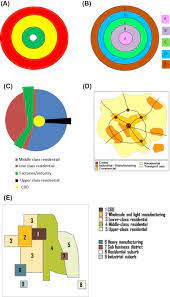
\includegraphics{fig/urban-structure.jpeg}
    \caption[Classical models of urban structure.]{There are several classical models of urban structure including Burgess' concentric zone model, Hoyt's sector model, and the multiple nuclei model described by Ullman and Harris. There's also been substantial work mapping particular patterns in particular cities. This model is more or less agnostic to the urban form, however there are interesting links and feedback loops to explore, mapping it to particular spatial forms, as discussed in Appendix~\ref{appendix-future-work} on Future Work.}
    \label{fig-urban-structure}
\end{figure}
% classical models of urban structure
% Burgess - concentric zone model
% Hoyt - sector model
% Ullman and Harris - multiple nuclei model
% and bid rent theory
% dis-amenity as well as amenity
% SLIDES https://slideplayer.com/slide/4208853/
% http://geographylaunchpad.weebly.com/economic-activity-in-urban-areas.html
% central place theory,  - cervices and centers attract places and compete with each other. - centers have a reach, 
% measure of centrality, and surounding hinterland - the max distance to use a service, has a threshold which is who is needed. 

\section{Summary}
In this chapter we have described stylized models, establishing how the urban system generates rents. % and relating them to neoclassical growth theory.  
% This chapter introduces the background to the theory of the urban model. 
This is important because we will essentially build that standard urban model into our model of financialization and in the process we will be adding to the standard urban model the distributional consequences that have been overlooked, by carrying the concept of rent through to explore the distributional consequences and how the distribution of rents feeds back into the productivity of cities. 

% Our base model builds on this basic classic urban Alonso model, so it will capture core features with a simple established framework to connect with the existing literature.  One feature of this model is that none of the simplifying assumptions are essential. We maintain the basic simplicity, but the mode can easily be generalized in many ways, and there is a substantial body of work extending and varying each of the simplifications in the model, as discussed above, as well as substantial work grounding and testing the model empirically.